\begin{figure}[H]
    \centering
    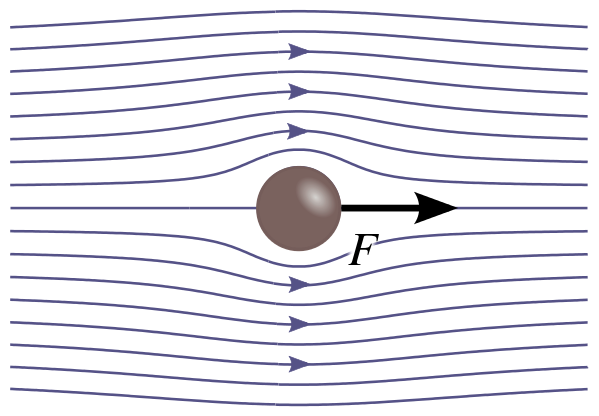
\includegraphics[width=10cm]{Flow Pattern.svg}
	\caption{{Diagram of the experiment carried down in this investigation}}
    \label{exp1}
\end{figure}


{Using the materials specified in chapter \ref{mat}, arrange the components as specified in figure \ref{exp1} and make sure that the spherical mass is kept about at a fixed point.}

{Following which, pass through the fluid in a rectangular chamber while varying temperatures and obtain the drag force eminent on the spherical mass.}

{After the prior setup and during the experiment, the fluid must interact with the spherical mass in a manner depicted in figure \ref{exp1}.}

